\documentclass[10pt, twocolumn]{scrartcl} % use larger type; default would be 10pt

\usepackage[utf8]{inputenc} % set input encoding (not needed with XeLaTeX)
\usepackage[cm]{fullpage}
\usepackage{amsmath}
\usepackage{caption}
\usepackage{float}
\usepackage{graphicx} % support the \includegraphics command and options
\usepackage[backend=biber]{biblatex} % use biber command to regenerate references
\usepackage{subcaption}

\renewcommand{\bibfont}{\footnotesize}
%\pagenumbering{gobble}
\usepackage{hyperref}
\addbibresource{report.bib}

\title{Accurate Vision-Based Landing For Multicopter UAVs}
\subtitle{CS287: Project Report}
\author{Constantin Berzan, Sunil Shah}
\date{} 

% TODO: say our code is open source at <url>

\begin{document}
\maketitle

\begin{abstract}
Multicopter UAVs have become increasingly popular over the last five years and are being considered for commercial purposes. However, they are hampered by their limited battery life. This class project is part of a larger project to build an automatic charging station for multicopters. Currently openly available automated landing algorithms rely on GPS to localise the UAV with respect to the landing station. We show that this approach is considerably inaccurate and implement a vision-based landing system which uses pose estimates to more accurately localise the UAV. 
In order to land based on this data, we build a state machine and controller that interacts with the open source ArduCopter autopilot to bring a test quadcopter down to a landing pattern. While environmental conditions and hardware issues ultimately prevented us from realising a vision-based landing, we are confident that, in good conditions and with some slight modification, our system should be able to land with much greater accuracy than GPS.
\end{abstract}
%%%%%%%%%%%%%%%%%%%%%%%%%%%%%%%%%%%%%%%%%%%%%%%%%%%%%%%%%%%%%%%%%%%%%%%%%%%%%%
\section{Motivation}
%% SUNIL
%% What is the problem? Why does it matter?
In the recent past, multicopter UAVs (or drones, as they are colloquially known) have become increasingly popular. This has been well documented by both mainstream and technology media. Once the preserve of the military, several factors have led to multicopter UAVs being fabricated and flown by hobbyist pilots:
\begin{description}
\item[The Maker Movement]{Affordable 3D printing has made it easier to prototype and produce cheap multicopter airframes.}
\item[Commodity Embedded Electronics]{A number of projects, beginning with the Arduino platform, have made well supported embedded computers available at low cost to the general public.}
\item[Open Source Software]{There are a number of popular open source autopilot projects that have significantly lowered the barrier to entry to novice users.}
\item[Smartphone IMUs]{As smartphones have grown in popularity, it has become possible to source low cost inertial measurement units (IMUs) which measure acceleration along one or more axes.}
\item[Ease of Control]{Multicopter UAVs offer the vertical take off and landing versatility of a traditional rotorcraft but with increased ease of control.}
\end{description}

These factors allow UAVs to be bought off the shelf for less than a thousand dollars, which is several orders of magnitude less than the cheapest traditional UAV. As with any disruptive technology, there is growing interest in the potential commercial applications. 

However, before these craft can be used reliably in a commercial setting, there are a number of shortfalls. In particular, accuracy of landing remains limited because of a reliance on GPS to localise the UAV. Our project aims to address this particular problem.


\subsection{Landing With GPS}
The de facto method of state estimation for outdoor UAVs is through sensor fusion of IMU data, barometric pressure measurements, and GPS data. IMUs are used to provide estimates of the UAV's roll, pitch and yaw rates and barometric pressure estimates the UAVs altitude. GPS data is used to geographically localise the UAV. Our experiments showed that using the auto-landing functionality (in \textit{return to launch} mode) of our autopilot resulted in an accuracy of landing that tracks the known accuracy of GPS systems. 

We experimentally gained 10 estimates for landing accuracy by drawing an X marker using yellow tape, arming the UAV at that location, flying it an arbitrary distance away and then invoking the \textit{return to launch} mode. We measured the straight line distance between the centre of the quadcopter and the centre of the marker. These results are shown in Table \ref{tbl:landing-data}, giving a mean accuracy of 195.33 centimetres and a standard deviation of 110.73 centimetres. 

\begin {table}
  \centerline{
  \begin{tabular}{ | c | c | }
  \hline
  Inches & Centimetres \\ 
  \hline
  22 & 55.88 \\ 
  63 & 160.02 \\ 
  39 & 99.06 \\ 
  84.5 & 214.63 \\ 
  25.5 & 64.77 \\ 
  76 & 193.04 \\ 
  158 & 401.32 \\ 
  130.5 & 331.47 \\ 
  76 & 193.04 \\ 
  94.5 & 240.03 \\ 
  \hline
  \end{tabular}}
   \caption{Distance of landing from home location using RTL}
   \label{tbl:landing-data}
\end {table}

\subsection{Accurate Landing}

Accurate landing is important for many applications of UAVs where it is necessary to land in and take off from constrained spaces. An example application is the use of UAVs as delivery vehicles to households. Many households may have limited clear space for the UAV to land. When using GPS, it is equally likely that the UAV will land on the household's roof as on their designated delivery point.

Accurate landing capability will also be an integral part of a larger project to build a multicopter charging station. Multicopters are limited by their battery life and current charging solutions require human intervention - which limits their usefulness as fully autonomous robots.  With an accurate landing, it becomes feasible to build an automatic conductive charger which can recharge a UAV's battery quickly.

\begin{figure*}[h]
    \centering
    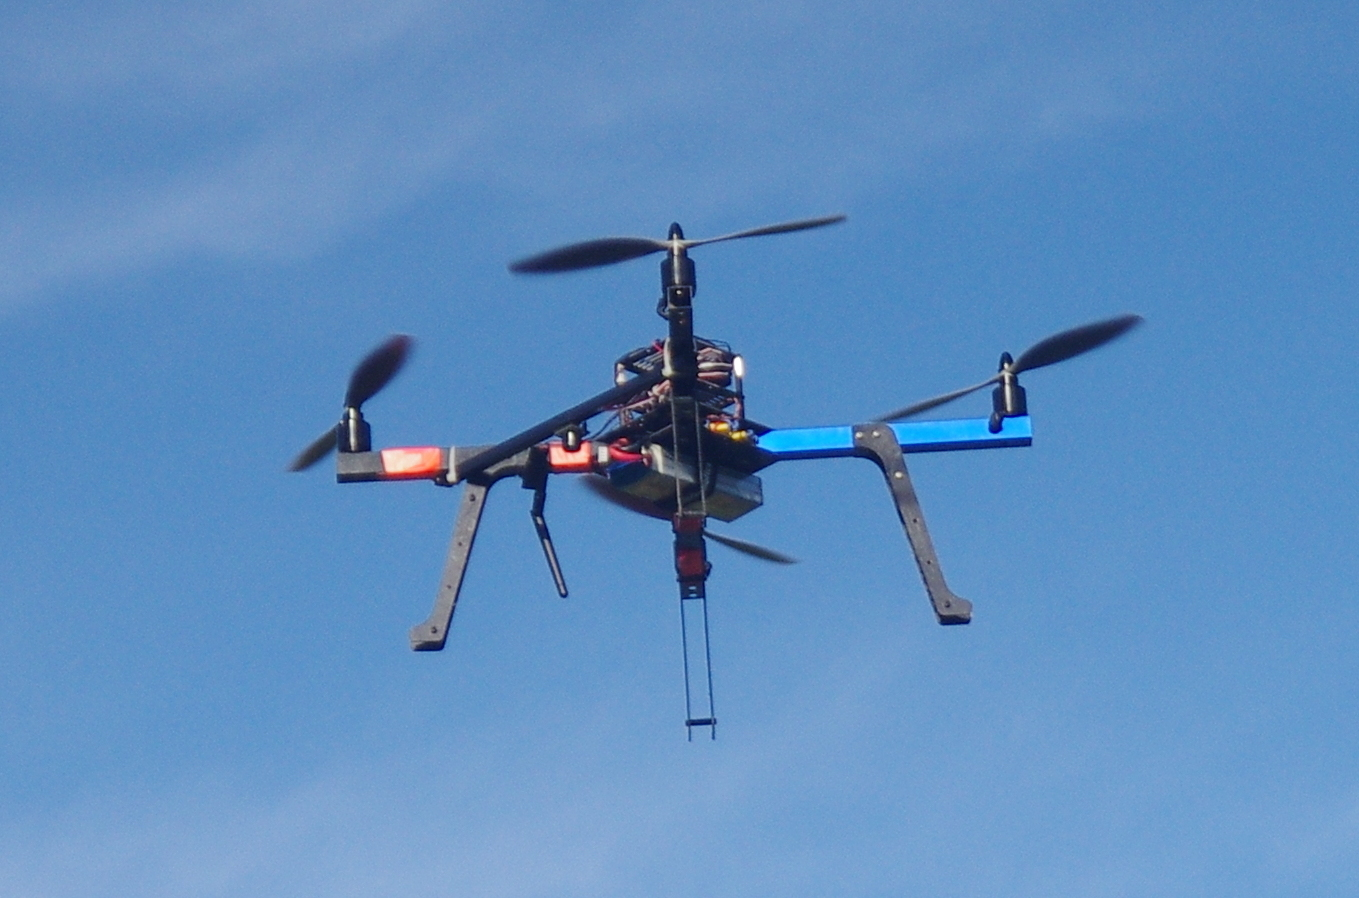
\includegraphics[width=\textwidth]{images/drone.jpg}
    \caption{Our test quadcopter in action.}
    \label{fig:drone}
\end{figure*}

\subsection{Vision-Based Landing}
By augmenting our autopilot with an additional computer and webcam, we can use computer vision techniques to gain a highly accurate estimate of the UAVs pose with respect to a landing pad of a known design.
Our project was thus to:
\begin{enumerate}
\item{Implement a vision-based pose estimator.}
\item{Integrate our pose estimates into a controller that would land a UAV.}
\item{Demonstrate accurate autonomous landing using commodity electronics on a low cost quadcopter UAV.}
\item{Make our software and implementation details openly available.}
\end{enumerate}

\section{Prior Work}

The automated landing problem has been investigated in the research literature
of the early 2000s. Here we briefly describe the approaches taken by some of
the most cited papers on this topic.

Sharp, Shakernia, and Sastry \cite{sharp_et_al_2001} designed an approach for
automatically landing an unmanned helicopter. Their landing target uses a
simple monochromatic design made up of several squares. Onboard the helicopter,
they use a pan-tilt-zoom camera and two embedded computers with Intel CPUs.
They discuss the details of their approach to pose estimation, but omit the
details of the helicopter controller. Using a real-time OS and optimized custom
code, they are able to get their vision system to operate at a rate of 30 Hz.

Our own approach in this project is modeled after that of Sharp et al. The main
differences are that (1) we use cheap off-the-shelf hardware, rather than
research-grade hardware; (2) our camera is stationary, it is not capable of
panning or tilting; and (3) we use off-the-shelf software components such as
ROS and OpenCV, rather than writing all of our code from scratch.

Saripalli, Montgomery, and Sukhatme \cite{saripalli_et_al_2002} designed
another approach for automatically landing an unmanned helicopter. They use a
monochromatic H-shaped landing target. Their onboard vision system detects this
landing target and outputs the helicopter's relative position with respect to
it. This is sent wirelessly to a behavior-based controller running on a ground
station, which then directs the helicopter to land on top of the target. They
are able to run their controller at 10 Hz this way. They are also using a
high-accuracy differential GPS system, and it is not clear how much their
differential GPS and vision systems contribute to a successful landing.

Garcia-Pardo, Sukhatme, and Montgomery \cite{garcia_pardo_et_al_2002} look at a
more general problem, where there is no pre-specified landing target, and their
helicopter has to search autonomously for a suitable clear area on which to
land.

%% Add comment re: further work since (i.e. landing on an unstable surface / moving boat).

\section{Approach}

\subsection{Architecture}

\begin{figure}[h!]
    \centering
    \begin{subfigure}[b]{0.9\textwidth}
        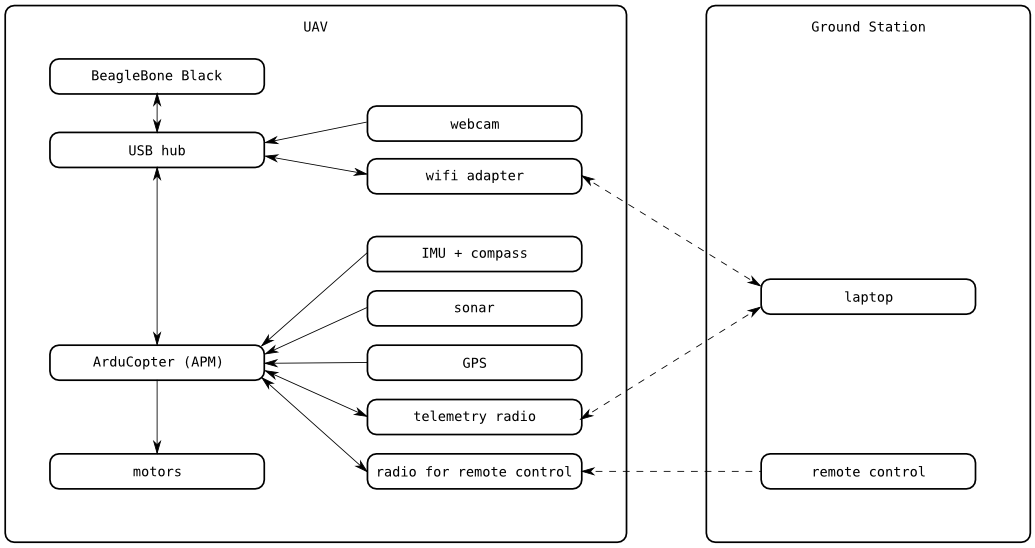
\includegraphics[width=\textwidth]{images/architecture.png}
        \caption{
            Architecture of our automated landing system. We use inexpensive
            off-the-shelf hardware. The laptop and remote control are for
            monitoring and emergency takeover by a human pilot. All the
            computation is performed onboard the UAV.
        }
    \end{subfigure}
    \\~\\
    \begin{subfigure}[b]{0.9\textwidth}
        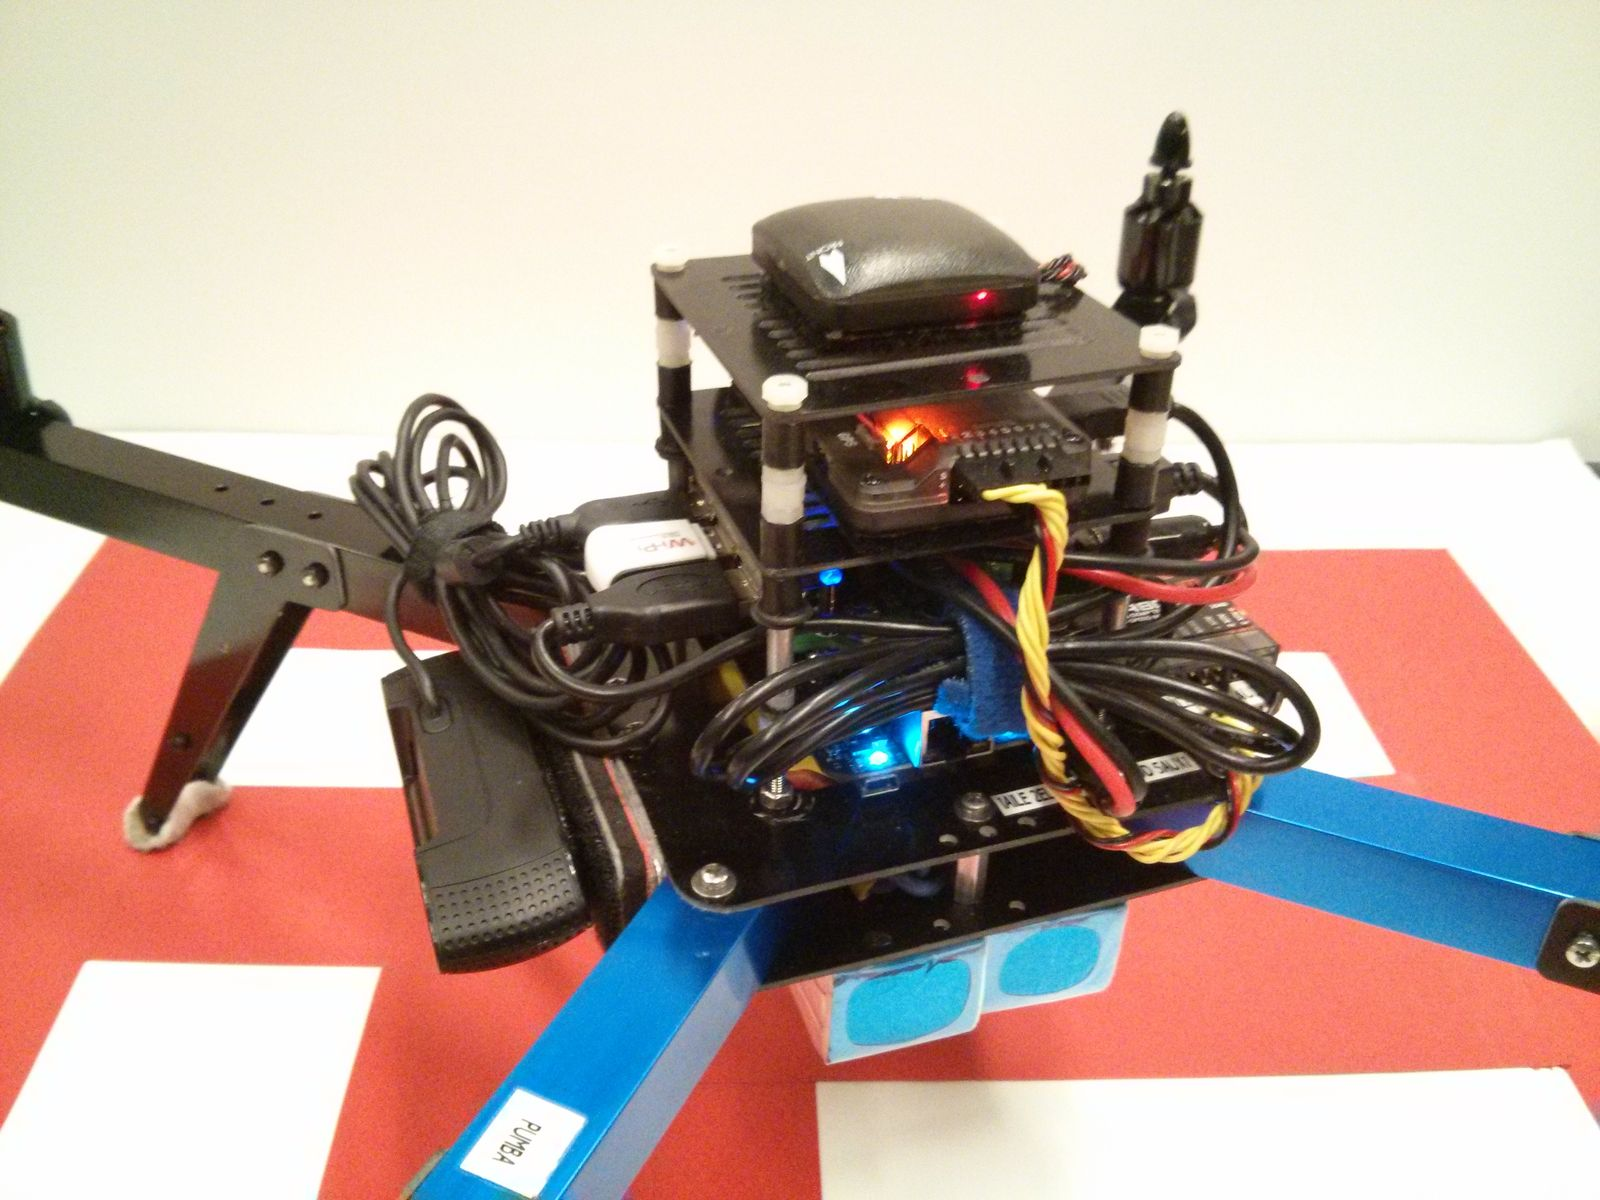
\includegraphics[width=\textwidth]{images/hardware.jpg}
        \caption{
            Our hardware stack fully assembled. From bottom to top: batteries,
            BeagleBone embedded computer, USB hub with Wi-Fi adapter, 3D
            Robotics autopilot (APM) with embedded sensors, GPS module. The
            webcam is on the left, and the radio for the remote control is on
            the right.
        }
    \end{subfigure}
    \caption{Hardware architecture and setup.}
    \label{fig:hardware}
\end{figure}

Our goal was to use inexpensive, off-the-shelf hardware, rather than expensive
equipment that is only accessible to researchers. We used quadcopter components
made by 3D Robotics, together with their ArduCopter autopilot (frequently
referred to under its old name -- Ardu-Pilot Mega, or APM) and associated GPS
module. This autopilot acts as a low-level controller that keeps the quadcopter
stable. It runs an unmodified version of the open-source autopilot code
provided by 3D Robotics.

We augmented the quadcopter with a BeagleBone Black embedded computer, which
uses a 1 GHz ARM CPU. (Since the ARM architecture is so different from x86,
the 1 GHz figure should not be compared to the frequency of modern-day Intel
CPUs, which are far more advanced, and expensive.) Using a powered USB hub, we
connected the autopilot to the BeagleBone. We also connected the webcam and a
Wi-Fi adapter this way.

% TODO:
% Weight of hardware stack?
% Estimated power consumption?
% Estimated cost of system?

On the BeagleBone, we installed a pre-built image of the Ubuntu 12.04
distribution, obtained from {\tt armhf.com}. We installed pre-built packages
for ROS groovy from the official ROS repositories. We compiled OpenCV 2.4.7 by
hand. We also installed roscopter, a third-party piece of software that reads
the state of the autopilot and makes it available via ROS, and also makes it
possible to send controls to the autopilot.


\subsection{Vision}
%% NAHUSH 
Our vision-based approach comprises of detecting corners of the squares on the 
landing platform and estimating the relative camera pose (position and orientation).

\subsubsection{Corner Detection}
%% NAHUSH
Thresholding and other chromatic approaches are largely dependent on the ambient light
and hence cannot be reliably used for accurate corner detection. Our approach is based
on detecting contours in the image. Following are the stages in our corner detection 
algorithm:

\begin{enumerate}
\item{Reduce noise in the image using a 3x3 median filter.}
\item{Detect edges using canny edge detector.}
\item{Identify contours and establish a tree-structured hierarchy among them.}
\item{Discard contours which are not four-sided convex polygons and which have an area
	less than an experimentally determined threshold value.}
\item{Using the contour hierarchy, determine a contour which contains 6 other contours.
	This contour represents the boundary of our landing platform. Store coordinates of
	the corners of these 6 inner contours. Move on to the next frame if we cannot detect 
	such a contour pattern.}
\item{Label the largest of the 6 polygons as 'A' and the farthest one from 'A' as 'D'.
	Label polygons as 'B', 'C', 'E' and 'F' based on orientations and distances relative
	to the vector formed by joining centers of 'A' and 'D' (vector DA) as shown in 
	Figure \ref{fig:corners}.}
\item{For each polygon, label corners in the anti-clockwise manner (Figure \ref{fig:corners})
	starting with the corner that belongs to the diagonal aligned with vector DA and that is 
	farther from D's center.}
\end{enumerate}

\begin{figure*}[h]
    \centering
    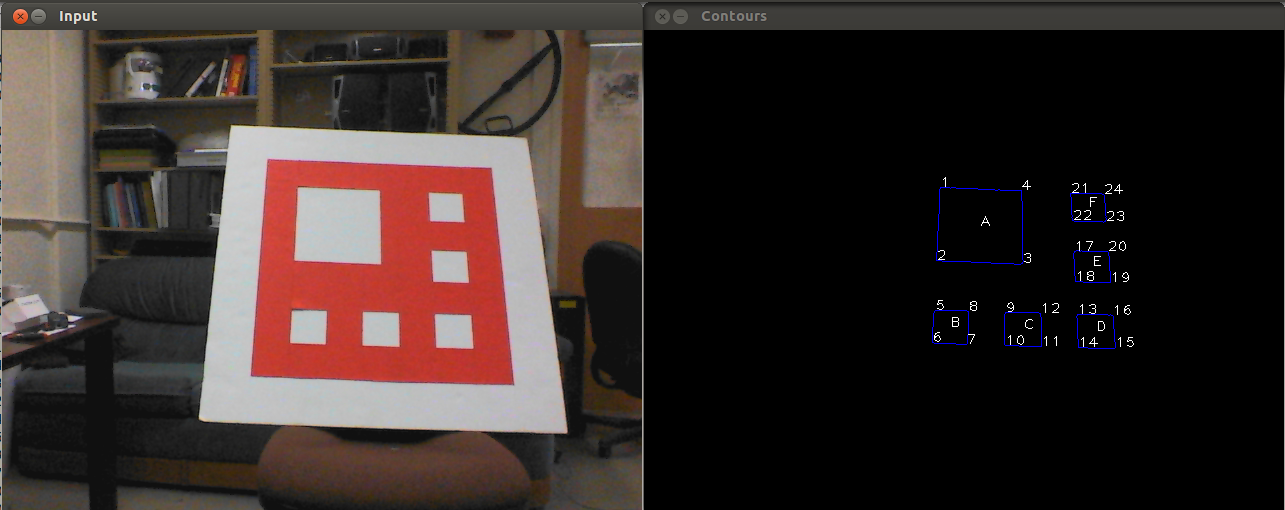
\includegraphics[width=\textwidth]{images/corners.png}
    \caption{Corner detection in action.}
    \label{fig:corners}
\end{figure*}

Note that we look for four-sided polygons and not specifically for squares, since they
will not appear as squares under perspective projection.

\subsubsection{Pose Estimation}

We define the origin of the world coordinate frame to be the center of the
landing platform, such that all points on the landing platform have a Z
coordinate of zero. The corner detector gives us image coordinates for the 24
corners. Thus, we have a set of 24 point correspondences between world
coordinates and image coordinates. Given this input, we want to compute the
quadcopter's pose, i.e. the position and orientation of the camera in the world
coordinate frame. To do this, we follow the approach of Sharp et al.
\cite{sharp_et_al_2001}.

% TODO: show math
% Have 48 equations (2 for each point pair)
% System of equations has 6 degrees of freedom

The output from the pose estimator is a translation vector
$t = \begin{bmatrix} t_x & t_y & t_z \end{bmatrix}^\top$
and a 3x3 rotation matrix $R$. We compute the camera position in world
coordinates as $C = -R^\top t$, and the yaw angle as
$\alpha = \arctan(R_{21} / R_{11})$. (The roll and pitch angles can be computed
similarly, but we do not require them in the control algorithm.)

The approach above assumes a calibrated pinhole camera. For the pose estimates
to be meaningful, our camera had to be calibrated first. We calibrated our
camera using the {\tt camera\_calibration} tool provided in the OpenCV
tutorials, plus some manual tuning. We used the resulting calibration matrix to
convert the raw pixel coordinates into coordinates for a calibrated pinhole
camera model, which we then fed into the equations above.


\subsection{Control}
%% SUNIl
In order to actually land our UAV using our pose estimates, it was necessary to implement a landing controller. Since this would need to run in real time (in order to adequately stabilise the UAV), we deferred real-time control to the \textit{loiter} mode provided by the ArduCopter autopilot. This takes care of real-time stabilisation for us and, additionally, attempts to keep the UAV in the same location using GPS. (They also offer a more basic stabilise mode which doesn't attempt to keep the craft to one location.)

Using the roscopter library, we were able to override the radio control inputs that would typically be received from the user. Using these inputs, we could manipulate the throttle, yaw, pitch and roll of the UAV.

%% TODO: Describe how we control the UAV using PWM values for channels.

\subsubsection{State Machine}
We designed a state machine with five states, beginning in a \textit{FLYING} mode and ending in \textit{POWER\_OFF}. Figure \ref{fig:statediagram} shows the transitions between the states. 

\paragraph{FLYING}
The \textit{FLYING} state represents when the UAV is not under our control, for instance, when the user is in manual control or has invoked another autopilot mode. Our controller listens to a specific channel of the radio input which represents three fixed values that are user selectable on the handheld transmitter. When the value of that channel changes to a predefined value, our controller takes control of the autopilot and transitions into \textit{SEEK\_HOME}.

\paragraph{SEEK\_HOME}
In \textit{SEEK\_HOME} mode, we use the built in \textit{return to launch} mode that ArduCopter implements - this navigates the UAV back to the launch location. Once above the launch location, the UAV should start receiving valid pose estimates.

\paragraph{LAND\_HIGH}
Our controller enters the \textit{LAND\_HIGH} mode when it starts receiving valid pose estimates. We use a simple proportional controller to calculate the appropriate control inputs based on the deviation from the centre of the landing station (in terms of x, y and yaw). These comprise the error terms in our controller.

Our controller disregards the z deviation and descends at a fixed rate. The z deviation is, however, used as the best estimate of altitude (our tests, described in section SECTION, show that the calculated z value is extremely accurate). When the UAV reaches a predefined altitude (where we know pose estimates will no longer be possible, due to field of view limitations), our controller enters into the \textit{LAND\_LOW} state.

\paragraph{LAND\_LOW}
In \textit{LAND\_LOW}, we use a dead reckoning approach to the ground since we are no longer able to receive valid pose estimates. Our controller attempts to keep the UAV flying straight and level and descends at a fixed rate. It uses data from the barometric pressure sensor to determine when the UAV has reached the ground and then enters into the \textit{POWER\_OFF} state.

\paragraph{POWER\_OFF}
\textit{POWER\_OFF} retains control of the UAV but sets throttle to a low value to prevent it from flying.

\begin{figure*}[h]
    \centering
    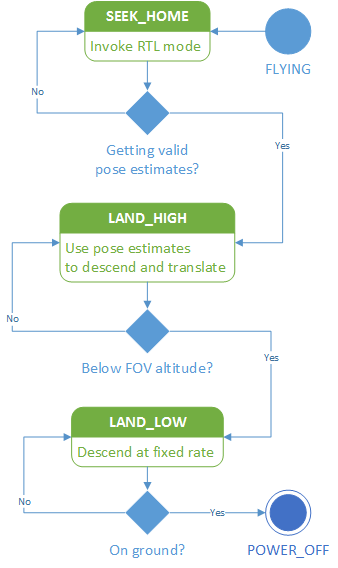
\includegraphics{images/statediagram.png}
    \caption{State diagram of our landing controller.}
    \label{fig:statediagram}
\end{figure*}

\subsection{Software Integration}
%% SUNIL
In order to integrate the three major components of software (roscopter, our pose estimator and our landing controller), we made extensive use of the publish and subscribe mechanism built into ROS. This allowed us to implement landing control in an event driven style - new control messages are generated upon receipt by the landing controller of new state information. This may include an updated pose estimate, an input from the user's radio control transmitter or new sensor data from the autopilot. Since the time taken to generate new control messages is considerably less than that to generate pose estimates, this allows us to generate control messages as frequently as we get new pose estimates. Figure \ref{fig:rosnodes} shows this setup.

\begin{figure*}[h]
    \centering
    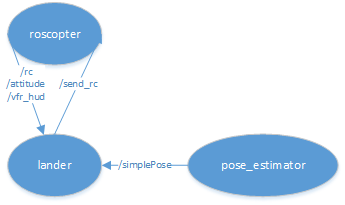
\includegraphics{images/rosnodes.png}
    \caption{Setup of our ROS nodes.}
    \label{fig:rosnodes}
\end{figure*}

\section{Results}

\subsection{Pose Estimation Accuracy}

We tested the accuracy of our pose estimator in the lab, by holding the camera
above the landing pad, and comparing the true measured height to the height
reported by the pose estimator. We also measured the standard deviation in our
pose estimate, by taking multiple measurements of the same scene. We compared
the standard deviation on x and y to the lower bound given by the dimensions on
the ground plane that correspond to one pixel in a 640x480 image at a given
height. Table \ref{tab:pose-accu} shows these results. There is a small (1.4\%
relative) systematic overestimation of the true height. This can be corrected
by doing more precise calibration. The height estimate is very stable at these
heights (small standard deviation). The x and y estimates are also fairly
accurate, although the error in these estimates is an order of magnitude
greater than the lower bound. This is consistent with the fact that there is
some noise in the corner detection, and the pose estimator finds an approximate
solution. In summary, this experiment suggests that our pose estimates should
be good enough to reliably land our quadcopter. If individual measurements are
too noisy, it is possible to get better pose estimates using a Kalman filter,
although that requires having a model of the dynamics and controls of the
system.

\begin{table}[h!]
    \centering
    \begin{tabular}{c|cc|cc|cc|c}
        true height & z mean    & z std     & x bound   & x std     & y bound   & y std     & yaw std \\
        \hline
         88 cm      & 89.3 cm   & 0.05 cm   & 0.19 cm   & 0.43 cm   & 0.14 cm   & 0.39 cm   & 0.12 $^{\circ}$ \\
        120 cm      & 121.1 cm  & 0.08 cm   & 0.26 cm   & 1.16 cm   & 0.19 cm   & 1.06 cm   & 0.12 $^{\circ}$ \\
        170 cm      & 172.0 cm  & 0.18 cm   & 0.37 cm   & 2.74 cm   & 0.27 cm   & 2.17 cm   & 0.07 $^{\circ}$ \\
        226 cm      & 229.0 cm  & 0.54 cm   & 0.49 cm   & 6.51 cm   & 0.36 cm   & 6.05 cm   & 0.34 $^{\circ}$ \\
    \end{tabular}
    \caption{
        Accuracy of our pose estimates. ``x bound'' and ``y bound'' are lower
        bounds for the error on x and y, given by the limited image resolution.
    }
    \label{tab:pose-accu}
\end{table}

\subsection{Performance}

When running on a modern-day laptop, our system easily achieves 30 frames per
second (FPS), the upper bound dictated by the camera we are using.
Unfortunately, performance is much slower on the embedded BeagleBone computer.
Just capturing frames from the camera puts significant strain on the system,
and we are only able to get 11.2 FPS, even if we perform no processing on the
frames. Adding the pose estimation code reduces performance to 3.0 FPS, and
running roscopter at the same time further reduces performance to 1.6 FPS.
Table \ref{tab:fps} summarizes these results.

These disappointing performance numbers point to a fundamental tradeoff when
developing a system such as ours: One could use off-the-shelf software packages
like ROS and OpenCV, which reduce development time, or one could talk directly
to the hardware and write all the code from scratch, which guarantees top
performance. Sharp et al \cite{sharp_et_al_2001} achieved 30 FPS with their
custom-code approach. Our experience suggests that even a decade later, it is
impractical to achieve good performance if we rely too much on third-party
libraries.

\begin{table}[h!]
    \centering
    \begin{tabular}{lr}
        camera upper bound                      &   30 FPS \\
        just capturing frames                   &   11.2 FPS \\
        running pose estimation                 &   3.0 FPS \\
        running pose estimation + roscopter     &   1.6 FPS \\
    \end{tabular}
    \caption{
        Performance of the embedded system, in terms of how many frames per
        second we can process.
    }
    \label{tab:fps}
\end{table}


\subsection{Control}

%% SUNIL 
% How did our controller do?

\subsubsection{Transitions}

% Field of view of camera and size of landing pad meant no accurate Z estimates
% below ~ 2m.
% Noisy sensor data = state transitions wer edifficult

\section{Challenges}
One of the significant impediments to our project was integrating working hardware. In this section, we describe the issues we had and how they might be mitigated in the future.

\subsection{Integration of Hardware}

We spent an unexpectedly large amount of time dealing with hardware issues. The
first two USB hubs we tried did not work reliably with the BeagleBone, failing
to be recognized if they were plugged in at boot time. The first Wi-Fi adapter
we tried did not support ad-hoc networking, despite the manufacturer's claims
to the contrary. In addition, the hastily written documentation for roscopter
mentioned the {\tt --rate} parameter instead of {\tt --baud-rate}, leading to
baffling failures to communicate with the APM, until we dug into this
third-party code and found the problem.\footnote{We have released a corrected
and somewhat cleaned-up version of roscopter at {\tt
https://github.com/cberzan/roscopter}.}

Another issue was that our webcam tried to automatically adjust exposure and
focus, which led to unfocused or over-exposed images in the field. After
extensive trial-and-error, we figured out how to tell the hardware to keep the
exposure and focus at fixed values, but this required that we run an experiment
to determine these values each time we went to fly our quadcopter.

Our main lesson from this experience is that we should not underestimate the
amount of time it takes to assemble and validate a new hardware platform for
running experiments. It is doubtlessly much quicker to get started with a
platform that others have already validated, or to use a software simulation.

\subsection{Image Quality}
%% NAHUSH

\begin{figure*}[h]
    \centering
    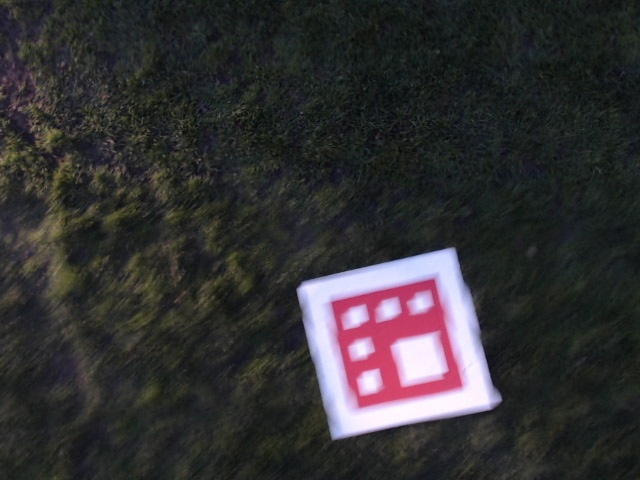
\includegraphics[width=\textwidth]{images/badimage.jpg}
    \caption{An example of a bad image.}
    \label{fig:badimage}
\end{figure*}

Since the multicopter is not inherently stable, images captured by the camera 
could be shaky (Figure \ref{fig:badimage}). 
Corner detection and hence pose estimation might not work on such blurry images. 
One of the possible ways of dealing with motion blur is using a better camera 
with more fine grained control.

\subsection{Field of View}
%% NAHUSH

\begin{figure*}[h]
    \centering
    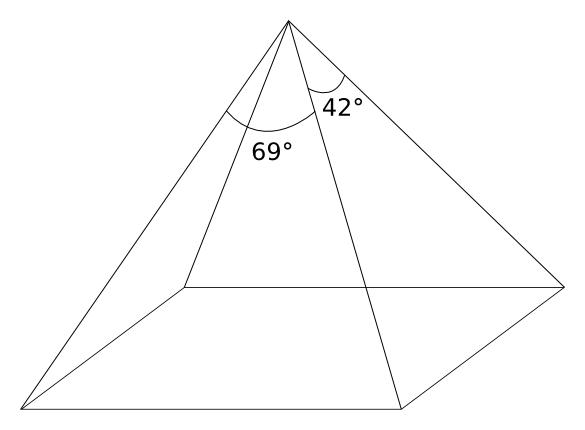
\includegraphics{images/fov.png}
    \caption{Field of view of our webcam.}
    \label{fig:fov}
\end{figure*}

The landing platform must entirely lie in the camera's field of view for the drone 
to get pose estimates. With our current setup, the drone needs to be at a height of 
at least 1 meter to be able to see the landing platform completely. 
Table \ref{tbl:visible-landing-area} shows the visible landing area corresponding to the 
drone's height from the ground.

\begin {table}[h!]
  \centerline{
  \begin{tabular}{ | c | c | }
  \hline
  Height & Visible Landing Area \\ 
  \hline
  1 m & 1.37 m x 0.77 m \\
  2 m & 2.75 m x 1.54 m \\
  4 m & 5.50 m x 3.07 m \\
  8 m & 11.0 m x 6.14 m \\
  16 m & 22.0 m x 12.3 m \\ 
  \hline
  \end{tabular}}
   \caption{Visible landing area from different heights}
   \label{tbl:visible-landing-area}
\end {table}

Since this field of view is measured with the camera centred above the landing pad, at 1 meter, we only generate pose estimates if the UAV is centred. In reality, it is not and so we typically lose pose estimates below approximately 2 meters. To mitigate this issue, we might reduce the size of the landing pad or explore using a concentric series of landing patterns.

\subsection{Weather}
%% SUNIL
The weather conditions became more limiting than we had initially imagined - in particular due to the short term nature of this project. 

\subsubsection{Temperature}
As mentioned in the Motivation section, multicopter UAVs have a limited battery life. The underlying battery technology is affected by the cold weather which meant that flight times, even with the largest 5500 mAh batteries on hand, were limited to 5 or 6 minutes. This limited the amount of testing per charge cycle.
Besides having a greater stock of batteries, there is little we can do to pre-empt this.

\subsubsection{Wind}
Our proportional controller struggled when there were large amounts of wind present. This is because it could not operate quickly enough to react to rapid changes in state, relying upon the \textit{loiter} mode of the autopilot to keep the UAV in the same place. The \textit{loiter} mode relies upon GPS to give us an estimate of the UAVs location and when the location deviates by a large amount, it tries to bring it back to the GPS location. As we've established, GPS is relatively inaccurate and so this causes a significant amount of drift.

This could be mitigated through better controller design. 

\paragraph{PID Controller}
Using a full PID controller will allow us to develop a more aggressive controller that is able to reduce the error (i.e. deviation from the centre of the landing pad) more quickly and in a way that is proportional to external noise (i.e. wind) - and not just the amount of noise.

\paragraph{Control Rate}
At the moment we gain pose-estimates at a slow rate (and provide control updates at the same rate) of approximately 1.6Hz. The GPS sensor used by the autopilot operates at 5Hz and is used to provide control updates at 10Hz. This is enough to control the quadcopter in real-time; increasing the performance of the pose estimator up to between 5 and 10Hz may be enough to better offset windy flying conditions.

\section{Conclusion \& Future Directions}

Use higher quality optics.
Explore landing pad design.
Allow landing in darker scenarios.
Use more advanced control loops (PID instead of just P).
Rewrite roscopter in C++.
Integrate sonar sensor for more accurate altitude estimates.

\printbibliography

\end{document}
